\subsubsubsection{biguint-sub}

\begin{enumerate}
    \item \verb|Target|: Implement the substraction of two biguints.
    \item \verb|Constraints logic|:
    \begin{itemize}
        \item Equation for gate;
        \item Sumcheck for ouptput;
        \item Rangecheck for limbs.
    \end{itemize}
    \item \verb|Circuit layout|: See \figref{fig:biguint-sub-circuit-layout}.
    \item \verb|Trace layout|: See \figref{fig:biguint-sub-trace-layout}.
    \item \verb|Constraints info and costs|:
    \begin{itemize}
        \item constraints-num: $6 \times (3 + 32 / 2) = 114$
        \item copy-constraints: $16$
        \item max-degree: $4$
        \item wires-num: $6 \times (5 + 16) = 126$
    \end{itemize}
\end{enumerate}

\begin{figure}[!ht]
    \centering
    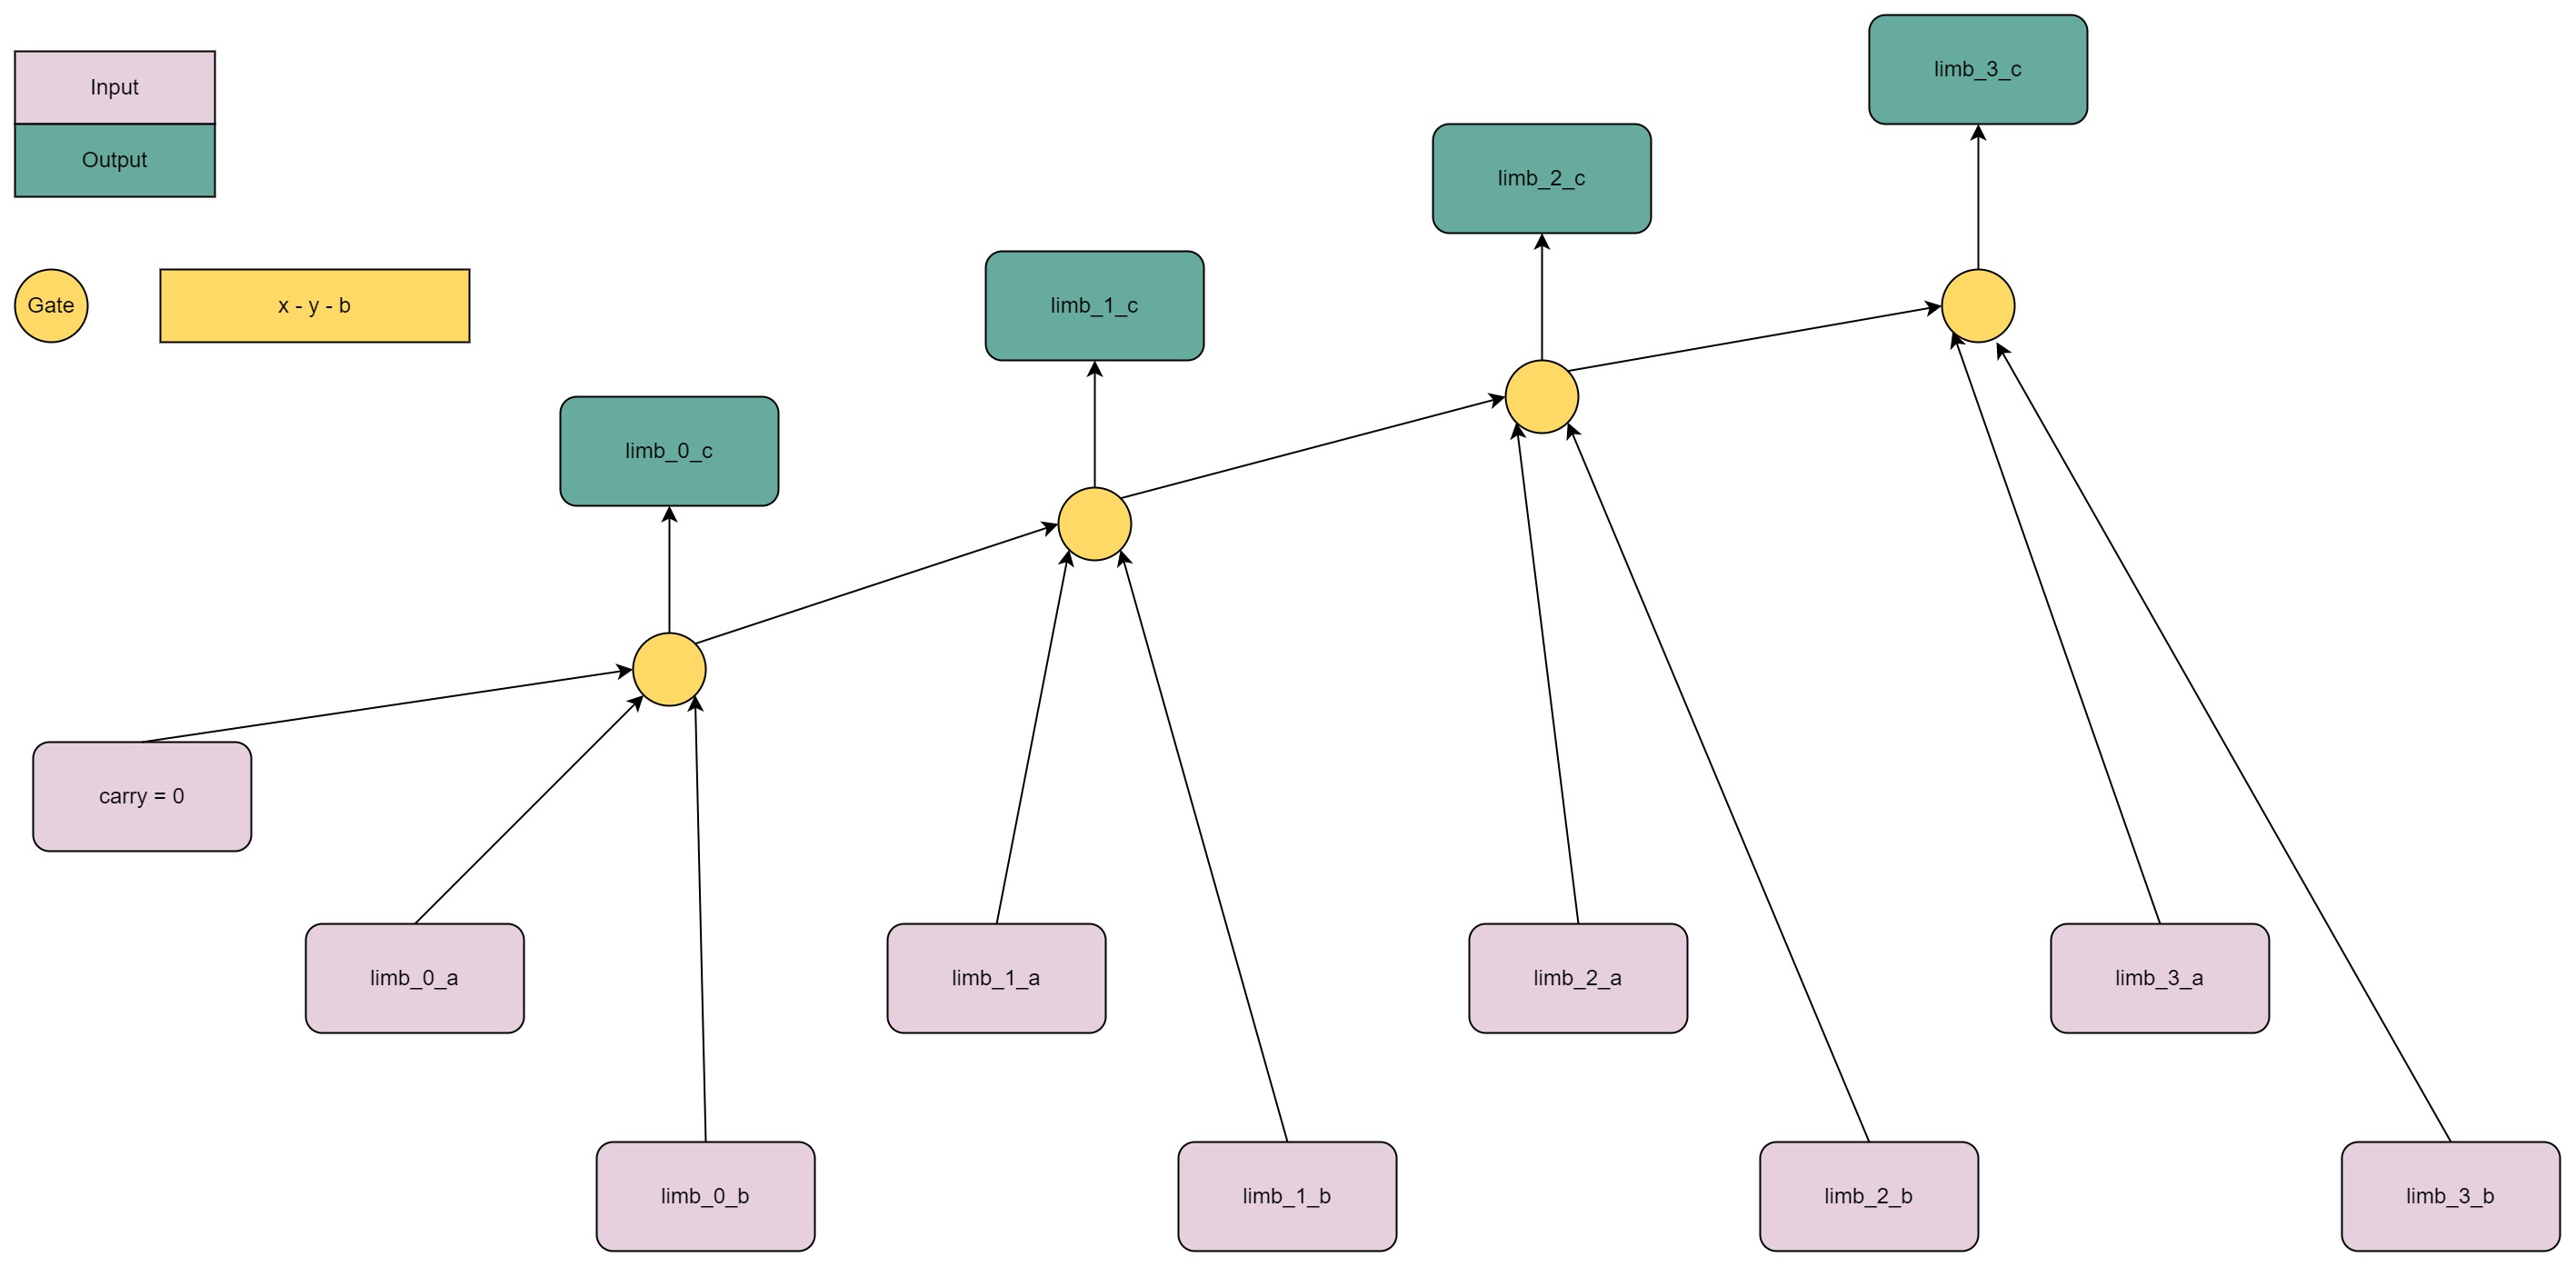
\includegraphics[width=0.6\textwidth]{biguint-sub-circuit-layout.jpg}
    \caption{biguint-sub circuit layout}
    \label{fig:biguint-sub-circuit-layout}
\end{figure}

\begin{figure}[!ht]
    \centering
    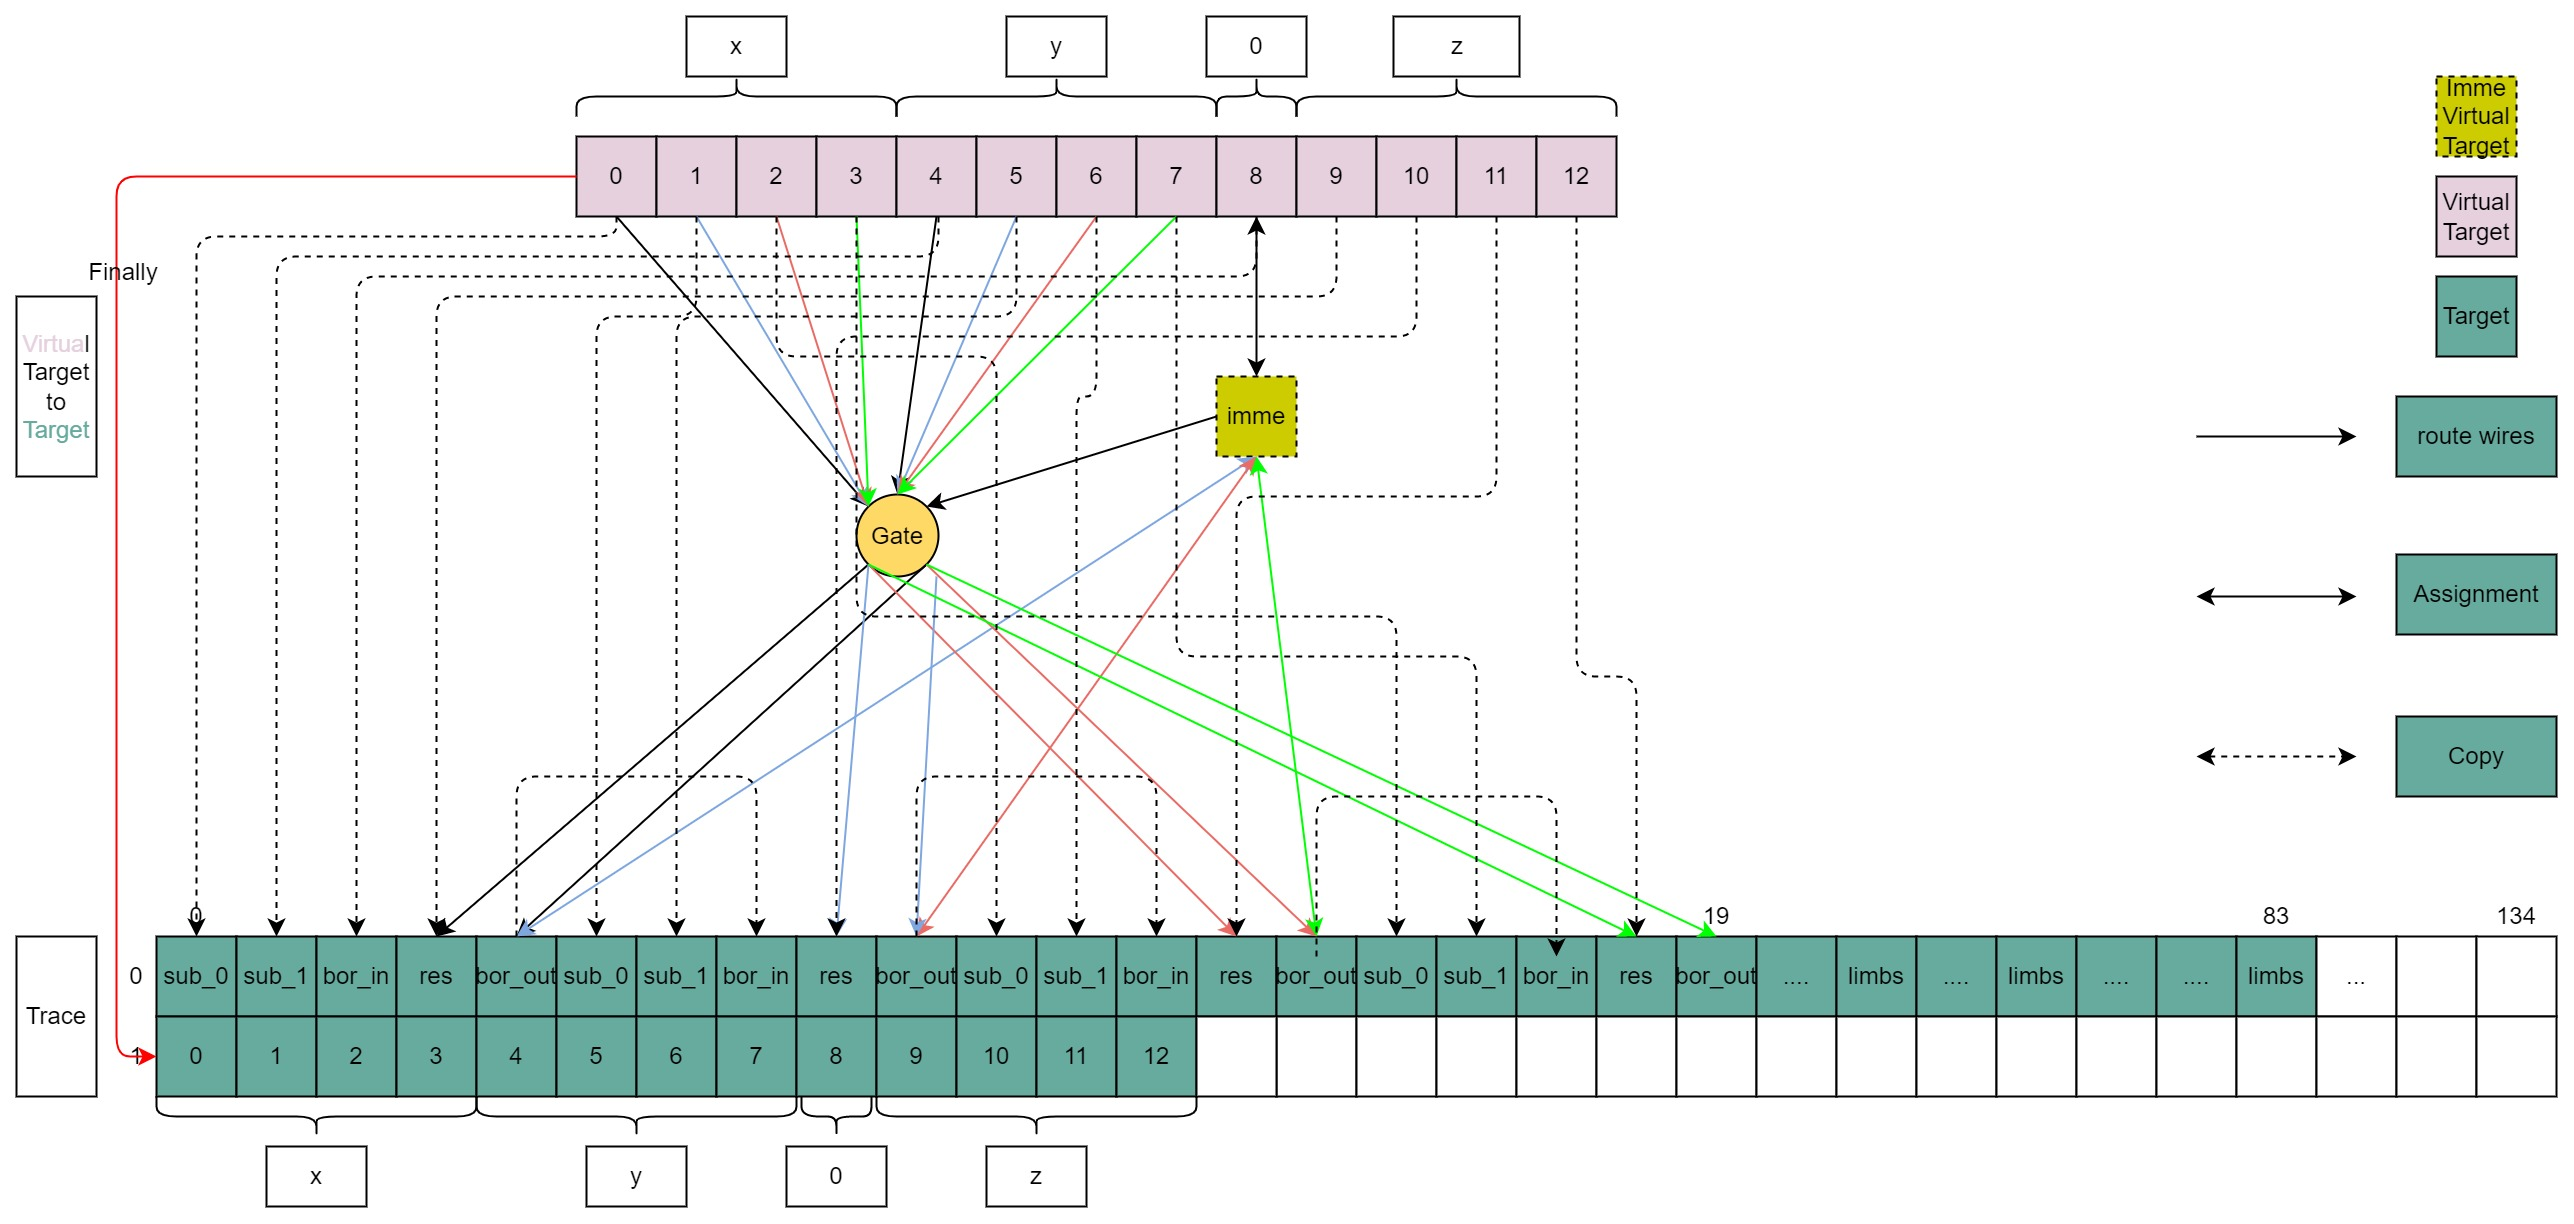
\includegraphics[width=0.6\textwidth]{biguint-sub-trace-layout.jpg}
    \caption{biguint-sub trace layout}
    \label{fig:biguint-sub-trace-layout}
\end{figure}
